\subsection{1}
\[
\begin{cases}
 4u_{tt} = u_{xx}+4t^{2} \cos(2x) \\ u|_{t=0} = e^{x}, \ u_{t}|_{t=0} = x^{2} 
\end{cases}
\] \\
\begin{gather*}
  u_{\text{частн}}= f(t) \cos(2x) \\ 
  4f'' \cos(2x) = -4f \cos(2x) +4t^{2} \cos(2x) \\ 
  f''=-f+t^{2} \\
  f = \alpha t^{2} + \beta t + \gamma \quad 2\alpha=-\alpha t^{2} - \beta t - \gamma + t^{2}\\ 
  \alpha = 1, \ \beta = 0, \ \gamma = -2 \\
  u_{\text{частн}} = (t^{2}-2) \cos(2x) \\
  u = (t^{2}-2)\cos(2x) + v(x,t) \\
  \begin{cases}
   4v_{tt}=v_{xx} \\ v|_{t=0}=e^{x}+2\cos(2x) \\ v_{t}|_{t=0} = x^{2} \\
  \end{cases} \\
  \boxed{v(x,t)= \frac{1}{2}(e^{x + \frac{t}{2}}+2\cos(2x+t)+e^{x -\frac{t}{2} }+2\cos(2x-t))
  + \int_{x- \frac{t}{2}}^{x +\frac{t}{2}} \xi^{2} \,d\xi} \\
\end{gather*}

\subsection{2}
$u_{tt}=a^{2}u_{xx}, \quad x \in \mathbb{R}^{1}, \quad t>0$ \\
\begin{enumerate}
  \item[\text{а})] $u|_{t=0}=\varphi(x), \ u_{t}|_{t=0}=0;$ \\
    \begin{gather*}
      \text{Ф-ла Даламбера} \\
      u(x,t) = \frac{\varphi(x+at)-\varphi(x-at)}{2} \\
    \end{gather*}
    \begin{minipage}{0.4\textwidth}
  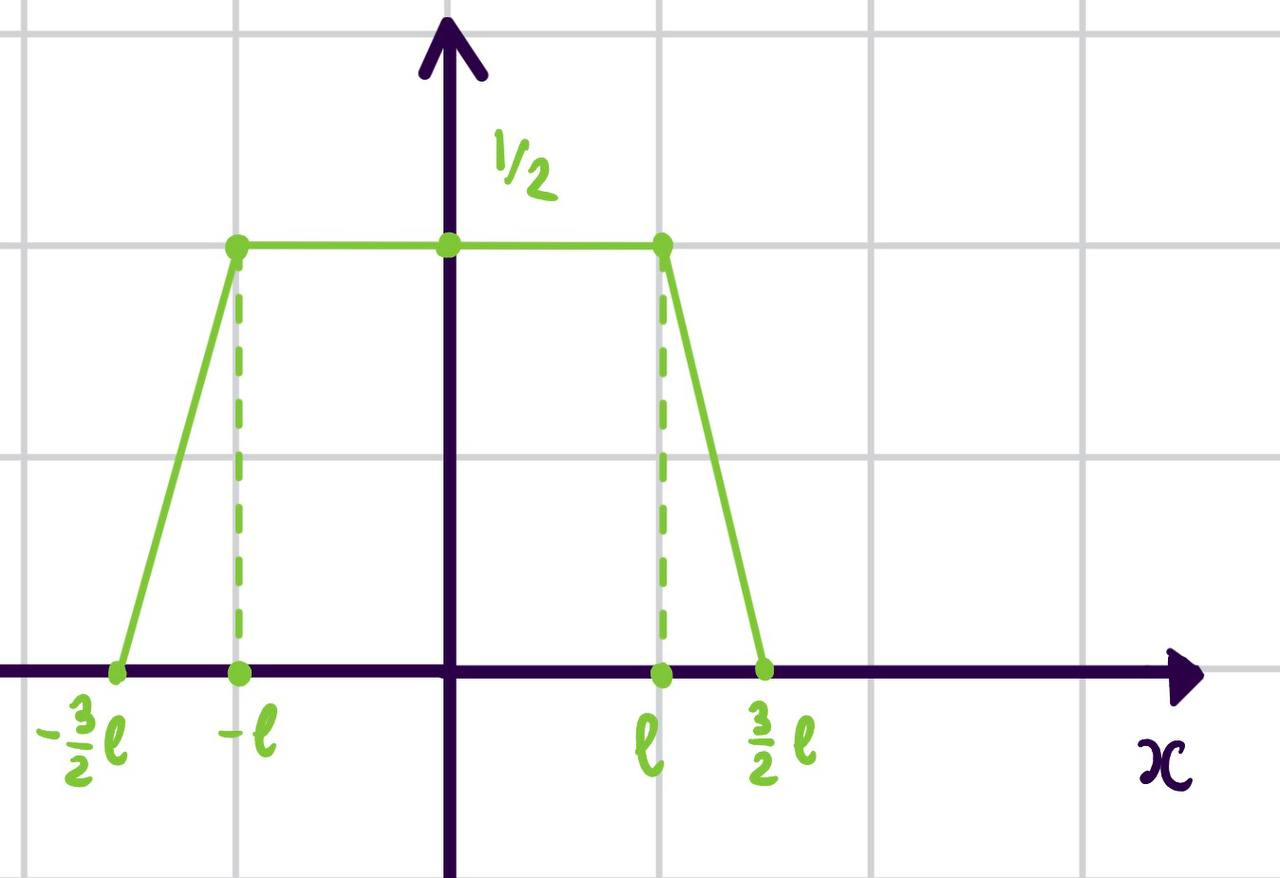
\includegraphics[width=1\linewidth]{pictures/u4.jpg} 
    \end{minipage}
    \begin{minipage}{0.4\textwidth}\raggedleft
      \begin{gather*}
        t = \frac{l}{2a} \\
        u(x,t) = \frac{\varphi(x+ \frac{l}{2})- \varphi(x -\frac{l}{2})}{2} \\
      \end{gather*}
    \end{minipage} \\
    \begin{minipage}{0.4\textwidth}
  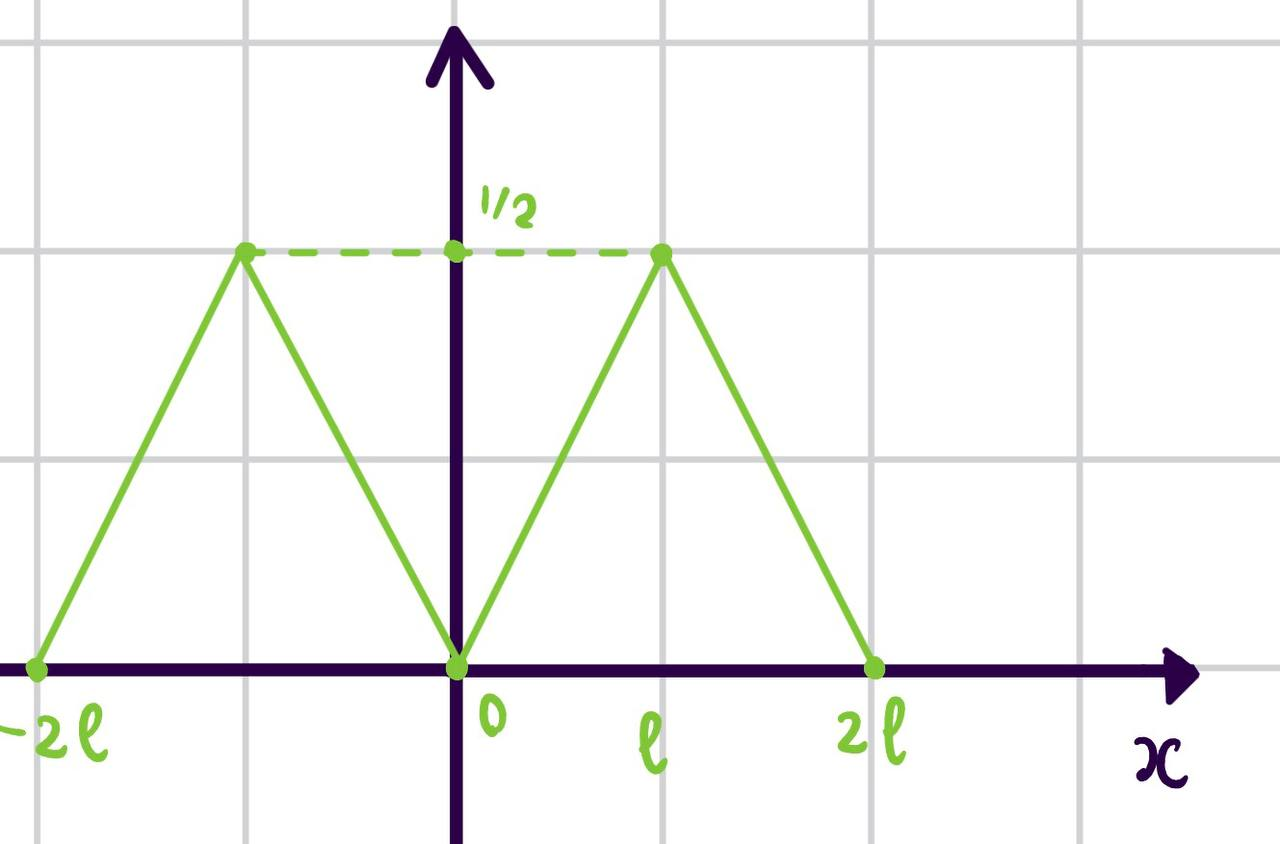
\includegraphics[width=1\linewidth]{pictures/u5.jpg} 
    \end{minipage}
    \begin{minipage}{0.4\textwidth}\raggedleft
      \begin{gather*}
        t = \frac{l}{a} \\
        u(x,t) = \frac{\varphi(x+ l)- \varphi(x -l)}{2} \\
      \end{gather*}
    \end{minipage} \\
    \begin{minipage}{0.4\textwidth}
  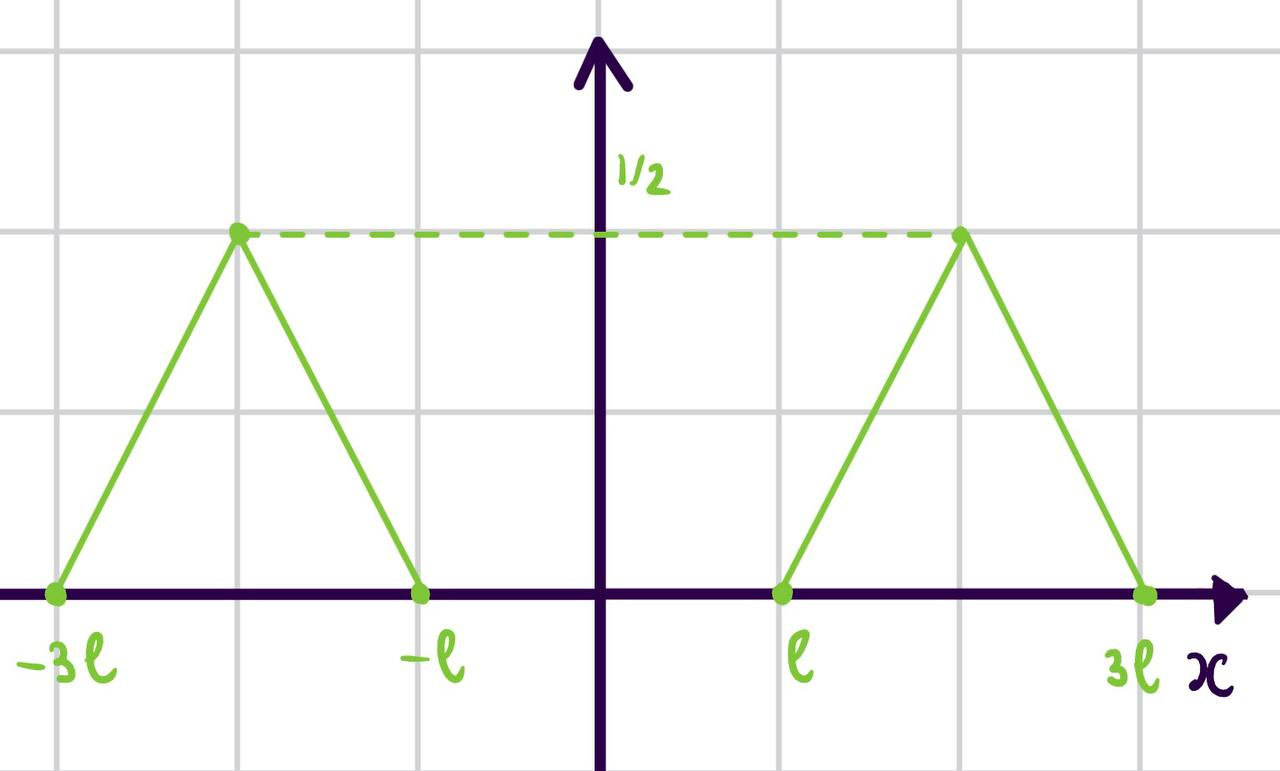
\includegraphics[width=1\linewidth]{pictures/u6.jpg} 
    \end{minipage}
    \begin{minipage}{0.4\textwidth}\raggedleft
      \begin{gather*}
        t = \frac{2l}{a} \\
        u(x,t) = \frac{\varphi(x+ 2l)- \varphi(x -l)}{2} \\
      \end{gather*}
    \end{minipage} \\
  \item[\text{б})] $u|_{t=0}=0, \ u_{t}|_{t=0}= \psi(x)=\theta(l-|x|) \\ 
    l = \text{const} >0 \quad \theta(x) = \begin{cases}
    1, \ x \geq 0 \\ 0, \ x < 0
  \end{cases}$ \\
  \begin{gather*}
    \text{Общее решение} \\
      u(x,t) = \frac{1}{2a}\int_{x-at}^{x+at} \psi(\xi) \,d\xi \\
  \end{gather*}
\end{enumerate}
    \begin{minipage}{0.4\textwidth}
  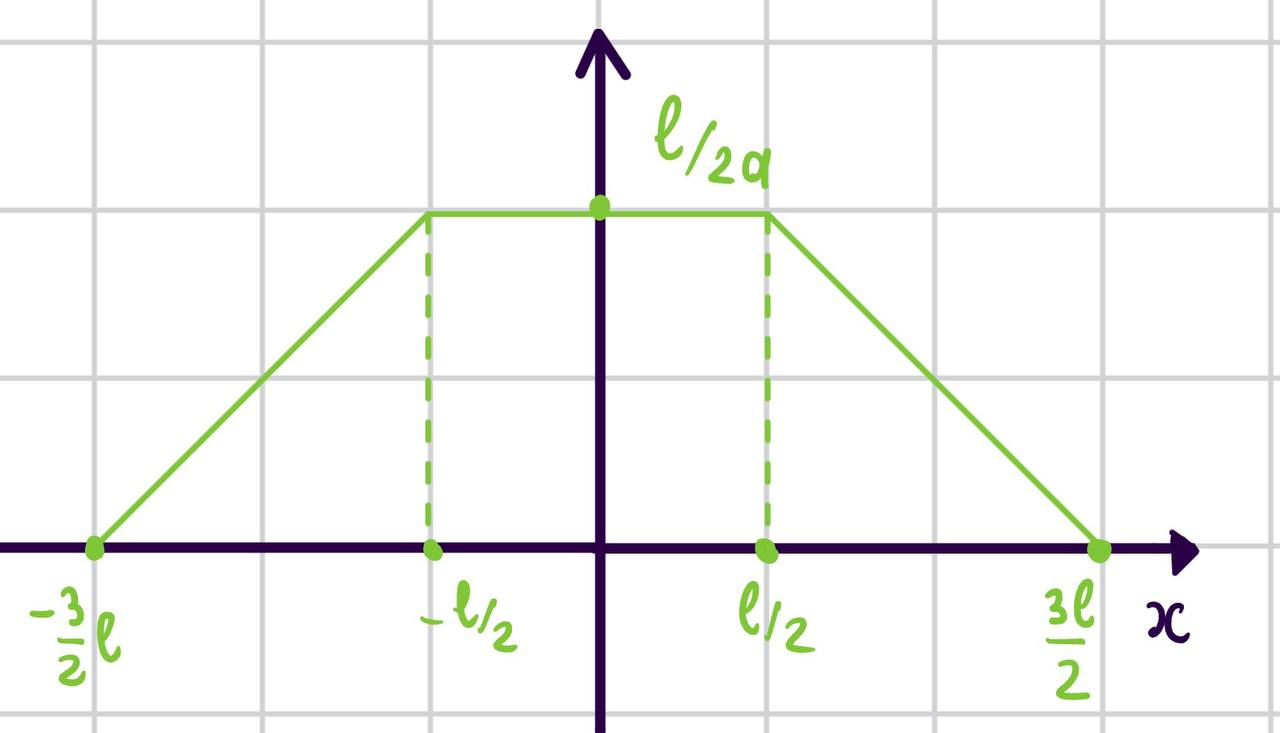
\includegraphics[width=1\linewidth]{pictures/u7.jpg} 
    \end{minipage}
    \begin{minipage}{0.4\textwidth}\raggedleft
      \begin{gather*}
        t = \frac{l}{2a} \\
        \begin{split}
        u(x,t) &= \frac{1}{2a} \int_{x- \frac{l}{2}}^{x + \frac{l}{2}} \theta(l -|\xi| )\,d\xi \\
               &= \frac{1}{2a} \text{length}\left([x-\frac{l}{2},x+\frac{l}{2}]\cap [-l,l]\right)
        \end{split}
      \end{gather*}
    \end{minipage} \\
    \begin{minipage}{0.4\textwidth}
  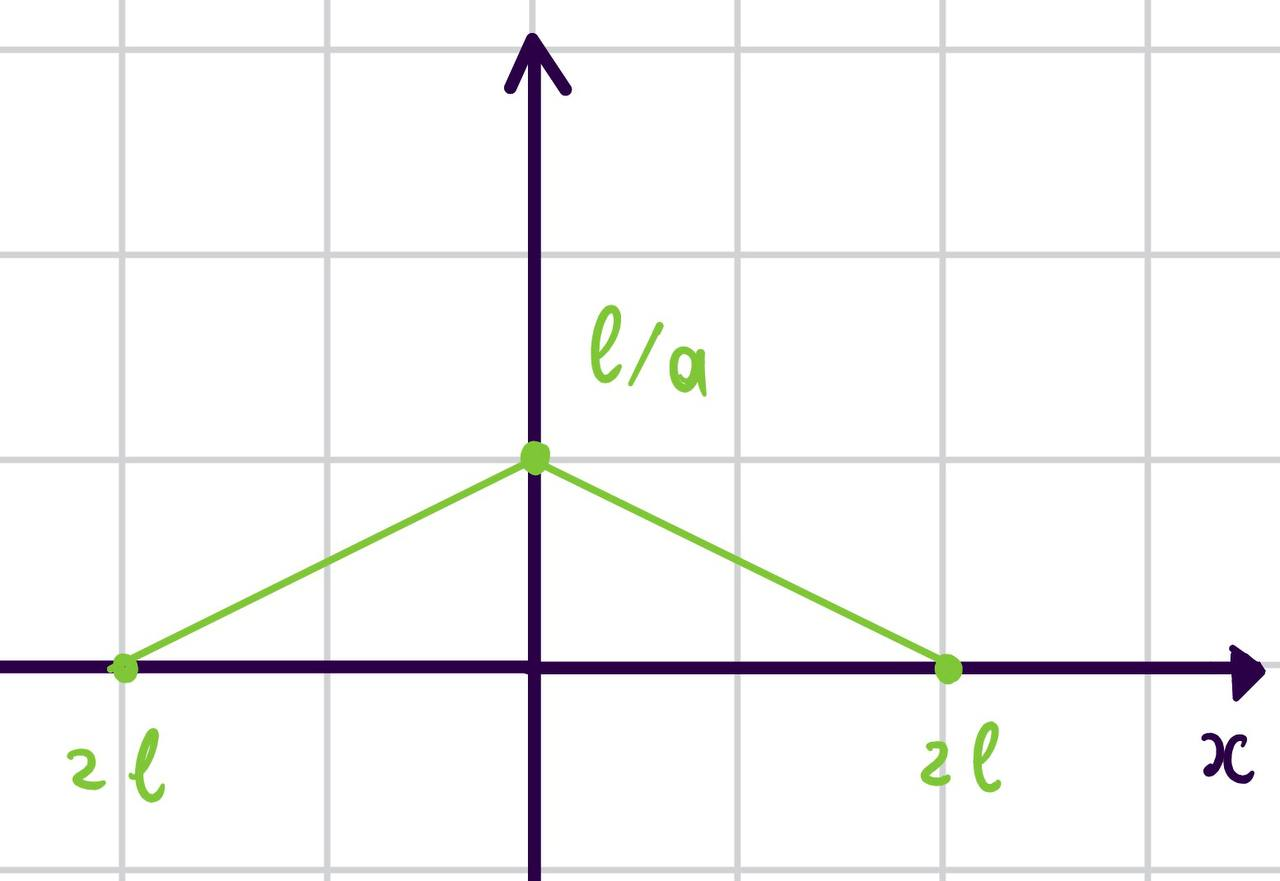
\includegraphics[width=1\linewidth]{pictures/u8.jpg} 
    \end{minipage}
    \begin{minipage}{0.4\textwidth}\raggedleft
      \begin{gather*}
        t = \frac{l}{a} \\
        \begin{split}
        u(x,t) &= \frac{1}{2a} \int_{x- l}^{x + l} \theta(l -|\xi| )\,d\xi \\
               &= \frac{1}{2a} \text{length}\left([x-l,x+l]\cap [-l,l]\right)
        \end{split}
      \end{gather*}
    \end{minipage} \\
    \begin{minipage}{0.4\textwidth}
  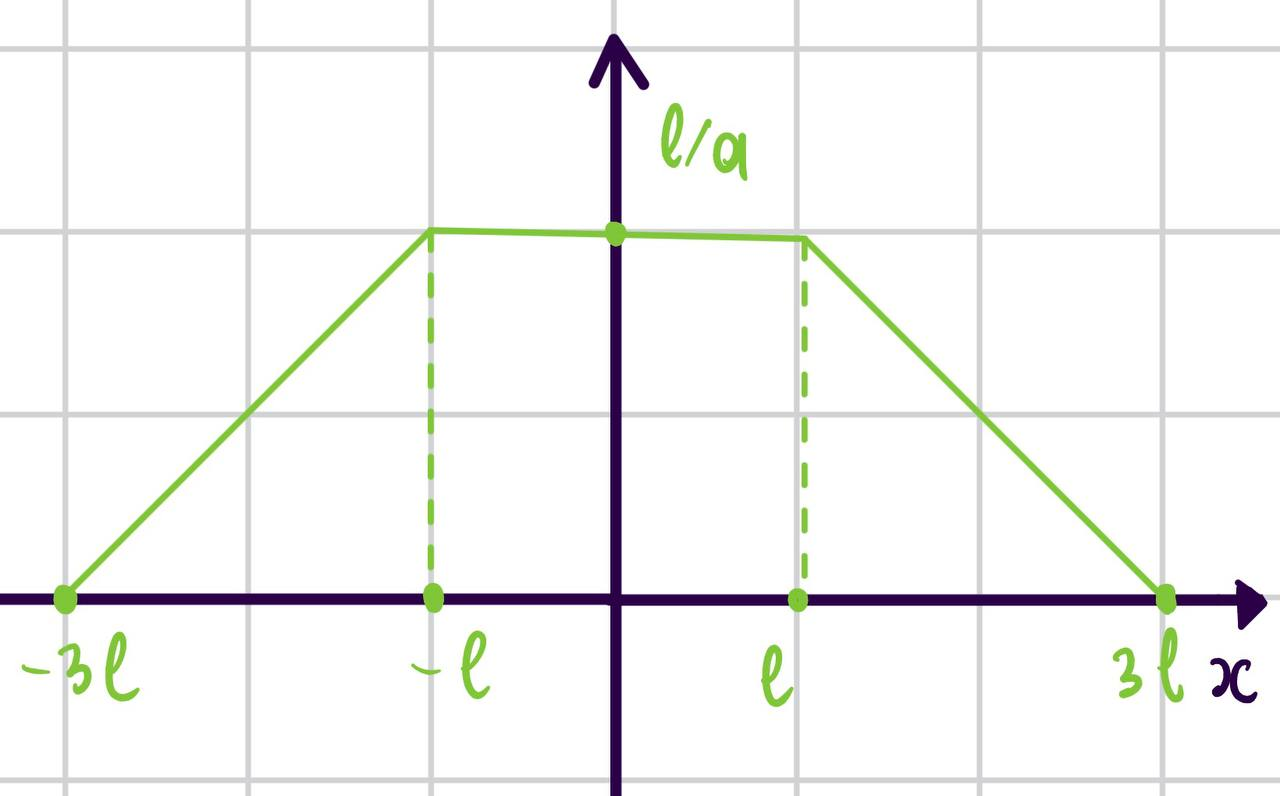
\includegraphics[width=1\linewidth]{pictures/u9.jpg} 
    \end{minipage}
    \begin{minipage}{0.4\textwidth}\raggedleft
      \begin{gather*}
        t = \frac{2l}{a} \\
        \begin{split}
        u(x,t) &= \frac{1}{2a} \int_{x- 2l}^{x + 2l} \theta(l -|\xi| )\,d\xi \\
               &= \frac{1}{2a} \text{length}\left([x-2l,x+2l]\cap [-l,l]\right)
        \end{split}
      \end{gather*}
    \end{minipage} \\
\subsection{3}
\begin{enumerate}
  \item[\text{а})] $21.19$ \\ $u_{tt}=3u_{xx}+2(1-6t^{2})e^{-2x}, \ t>0, \ x>0$ \\
    $u|_{t=0}=1, \ u_{t}|_{t=0}=x, \ (u_{x}-2u)|_{x=0}=-2+t-4t^{2}$ \\
    \begin{gather*}
      \text{Ищем частное решение} \\
    u_{\text{частн}} = e^{-2x}(At^{2}+Bt+C) \\
    2Ae^{-2x}=12e^{-2x}(At^{2}+Bt+C)+2(1-6t^{2})e^{-2x} \\
    2A=12At^{2}+12Bt+12C+2-12t^{2} \\
    \end{gather*} \\
    \begin{gather*}
    \begin{cases}
      A = 1, \\ B = 0, \\ C = 0;
    \end{cases} \\
    u_{\text{частн}} = t^{2}e^{-2x} \\
    \text{Сводим ур-е к однородному} \\
    u = t^{2}e^{-2x}+v(x,t) \\
    v_{tt}=3v_{xx} \\ v|_{t=0}=1, \quad v_{t}|_{t=0}=x, \quad
    (v_{x}-2v)|_{x=0}=-2+t \\
    v = f(x +\sqrt{3}t)+g(x-\sqrt{3}t) \\
    \text{Ищем решение в области $x \geq \sqrt{3}t$ }\\
    v|_{t=0}=f(x)+g(x)=1 \qquad v_{t}|_{t=0}=\sqrt{3}f'(x)-\sqrt{3}g'(x)=x \\
    f'(x)+g'(x)=0 \\
    2 \sqrt{3}f'(x) = x\\ 
    \boxed{f(x)= \frac{x^{2}}{4 \sqrt{3}} + C, \quad g(x) =1 - \frac{x^{2}}{4 \sqrt{3}} - C}\\
    v(x,t) = 1 - \frac{(x+ \sqrt{3}t)^{2}-(x - \sqrt{3}t)^{2}}{4 \sqrt{3}} = 1 -xt \\
    \text{Ищем решение в области $x < \sqrt{3}t$} \\
    (v_{x}-2v)|_{x=0}=f'(\sqrt{3}t)+g'(-\sqrt{3}t)-2f(\sqrt{3}t)-2g(-\sqrt{3}t)-2C=-2+t \\
    \text{Заметим, что уравнение полученное в области $x \geq \sqrt{3}t$ также подходит} \\
    \text{Следовательно, решения на полученных областях совпадают} \\
    \boxed{u(x,t)=1-xt+t^{2}e^{-2x}}\\
    \end{gather*} \\
    $21.2$ \\
    $u_{tt}-a^{2}u_{xx}=0$ \\
    $u|_{t=0}=u_{0}(x), \quad u_{t}|_{t=0} = u_{1}(x)$ \\
    $u_{x}|_{x=0}=0$ \\
    \begin{gather*}
      u(x,t)=f(x+at)+g(x-at) \\
      x \geq at \\
      f(x)+g(x)=u_{0}(x), \quad u_{t}|_{t=0}=af'(x)-ag'(x)=u_{1}(x) \\
      f(x)-g(x)= \frac{1}{a}\int_{0}^{x} u_{1}(\xi) \,d\xi+A \\
      f(x)= \frac{u_{0}(x)}{2}+ \frac{1}{2a}\int_{0}^{x} u_{1}(\xi) \,d\xi+\frac{A}{2} \qquad
      g(x)= \frac{u_{0}}{2}- \frac{1}{2a}\int_{0}^{x} u_{1}(\xi) \,d\xi-\frac{A}{2} \\
 \boxed{ u(x,t) = \frac{u_{0}(x+at)+u_{0}(x-at)}{2}+\frac{1}{2a}
 \int_{x-at}^{x+at} u_{1}(\xi) \,d\xi} \\
    x<at \\
    u_{x}|_{x=0} = f'(at)-g'(-at)=0 \Rightarrow f(at)+g(-at)=C \\
    g(-at)=C- \frac{u_{0}(at)}{2}=\frac{1}{2a}\int_{0}^{at} u_{1}(\xi) \,d\xi-\frac{A}{2} \\
    g(b)=C- \frac{u_{0}(-b)}{2}=\frac{1}{2a}\int_{0}^{-b} u_{1}(\xi) \,d\xi-\frac{A}{2} \\
    \text{Сшивка} \\
    g(+0)=g(-0) \\
    C-\frac{A}{2}=u_{0}-\frac{A}{2} \Rightarrow C = u_{0}(0)=0 \\
    \text{Показали, что} \\
    \boxed{u(x,t)= \frac{1}{2a}\int_{x-at}^{x+at} u_{1}(\xi) \,d\xi + \begin{cases}
      \frac{u_{0}(x+at)+u_{0}(x-at)}{2}, \ x \geq at \\
      \frac{u_{0}(x+at)-u_{0}(x-at)}{2}, \ x < at \\
  \end{cases}}
    \end{gather*} \\
  \item[\text{б})] $u_{tt} = u_{xx} +xe^{t}, \quad x>0,t>0$ \\
$u|_{t=0} = 1+x, \quad u_{t}|_{t=0} = 4-5x, x \geq 0$ \\
$(2u+u_{x})|_{x=0}=(1+t)e^{t}+2+t-3t^{2}, \quad t \geq 0$ \\
\begin{gather*}
  \text{Ищем частные решения} \\
  u_{\text{частн}} = xe^{t} \\
  \text{Сводим ур-е к однородному} \\
  u = xe^{t} + v(x,t) \\
  v_{tt} = v_{xx} \qquad v|_{t=0} = (u - xe^{t})|_{t=0} = 1+x-x=1 \\
  v_{t}|_{t=0}=(u_{t}-xe^{t})|_{t=0}=4-5x-x=4-6x \\
  (2v+v_{x})|_{x=0} = (2u+u_{x}-2xe^{t}-e^{t})|_{x=0} = te^{t}+2+t-3t^{2}, \ t \geq 0 \\
v = f(x+t) + g(x-t) \\
\text{Ищем решение в области $x \geq t$} \\
v|_{t=0} = f(x)+g(x) = 1 \qquad v_{t}|_{t=0} = f'(x) - g'(x) = 4 - 6x, \ x \geq 0 \\
f'(x) + g'(x) = 0, \qquad \text{складываем} \\
2f'(x)=4-6x \qquad 2f'(x) = 4-6x \qquad f'(x) = 2-3x \\
\boxed{f(x)=2x -\frac{3x^{2}}{2}+A; \qquad g(x) = 1-2x+ \frac{3x^{2}}{2}-A} \\
v = 2(x+t) - \frac{3}{2}(x+t)^{2}+A+1-2(x-t)+ \frac{3}{2}(x-t)^{2}-A, \ x \geq t \\
\text{Ищем решения при $x < t$} \\
\begin{split}
  (2v+v_{x})|_{x=0} &= 2f(t)+2g(-t)+ f'(t) + g'(-t) = \\
                    &= te^{t} +2+t -3t^{2}, \ t \geq 0 \\
\end{split} \\
4t-3t^{2}+2A+2g(-t)+2-3t+g'(-t) = te^{t}+2+t-3t^{2} \\
g'(-t)+2g(-t)=te^{t}-2A \qquad -t = p < 0 \\
\end{gather*}
\begin{gather*}
g'(p)+2g(p)=-pe^{t}-2A \\
  g_{\text{частн}_{1}} = (\alpha p + \beta ) e^{-p} \\
  \alpha e^{-p}- (\alpha p +\beta)e^{-p}+2(\alpha p + \beta)e^{-p} = -pe^{-p} \\
  \alpha +2\alpha = -1 \qquad \alpha = -1 \qquad \alpha - \beta +2 \beta = 0 \\
  \beta = -\alpha = 1 \\
  g_{\text{частн}_{1}} = (1-p)e^{-p} \qquad g_{\text{частн}_{2}}=-A \\
  g(p) = ce^{-2p}+(1-p)e^{-p}-A, \quad p < 0 \\
  \text{Сшивка(склейка)} \\
  g(+0)= g(-0) \\
  1-A=C+1-A \Rightarrow C = 0 \\
  \text{Ответ} \\
  \boxed{u(x,t)=xe^{t}+2(x+t)- \frac{3}{2}(x+t)^{2} +
  \begin{cases}
   1-2(x-t) + \frac{3}{2}(x-t)^{2}, \quad x \geq t \\
   (1-(x-t))e^{-(x-t)}, \quad x <t \\
\end{cases}}
\end{gather*}
\item[\text{в})] $4u_{tt}=u_{xx}-3\sin(x+t), \ x >0, \ t>0$ \\
  $u|_{t=0}=\sin(x)+\sin(2x),\quad u_{t}|_{t=0}=2+\cos(x), \ x \geq 0$ \\
  $(u_{x}-2u)|_{x=0}=2-4t-2\sin(t)+\cos(t), \ t \geq 0$ \\
  \begin{gather*}
    \text{Ищем частное решение} \\
    u_{\text{частн}} = \sin(x+t) \\
    \text{Сводим уравнение к однородному} \\
    u = \sin(x+t)+v(x,t) \\
    v_{tt}=\left(\frac{1}{2}\right)^{2}v_{xx}, \quad v|_{t=0}=\sin(2x), \quad v_{t}|_{t=0}=2 \\
    (v_{x}-2v)|_{x=0}=2-4t, \ t \geq 0 \\
    v = f(x+ \frac{t}{2})+g(x - \frac{t}{2}) \\
    \end{gather*} \\
    \begin{gather*}
    \text{Ищем решение в области $x \geq \frac{t}{2}$} \\
    v|_{t=0}=f(x)+g(x)=\sin(2x) \\
    v_{t}|_{t=0}= \frac{1}{2}f'(x)- \frac{1}{2}g'(x)=2 \\
    f'(x)+g'(x)=2\cos(2x) \qquad f'(x)=\cos(2x)+2 \\
    \boxed{f(x)= \frac{1}{2}\sin(2x)+2x+C,\quad g(x)= \frac{1}{2}\sin(2x)-2x-C} \\
      v(x,t)=\frac{1}{2}\sin(2x+t)+\frac{1}{2}\sin(2x-t), \ x \geq \frac{t}{2} \\
      \text{Область $x < \frac{t}{2}$} \\
      \left(v_{x}-2v\right)|_{x=0}=f'\left(\frac{t}{2}\right)+g'\left(-\frac{t}{2}\right)-2f\left(\frac{t}{2}\right)-2g\left(-\frac{t}{2}\right) = 
      2 - 4t\\
\cos\left(t\right)+2-2\left(\frac{1}{2}\sin\left(t\right)+t+C\right)+g'\left(-\frac{t}{2}\right)+g\left(-\frac{t}{2}\right)=2-4t \\
g'(b)+g(b)+\sin(2b)+\cos(2b)-4b-2C = 0, \quad b = - \frac{t}{2} \\
\text{Решая дифф. ур-е} \\
g(b)=Ae^{2b}-2b-1+\frac{1}{2}\cos(2b)-C \\
\text{Сшивка} \\
g(+0)=g(-0) \\
A-1+\frac{1}{2}-C=-C \Rightarrow A =\frac{1}{2} \\
\boxed{u=\sin(x+t)+\frac{1}{2}\sin(2x+t)+\begin{cases}
  \frac{1}{2}\sin(2x-t), \ x \geq \frac{t}{2} \\
\frac{1}{2}\cos(2x-t)+2t-1+\frac{1}{2}e^{2x-1}, \ x < \frac{t}{2}
\end{cases}} \\
\end{gather*} \\
\item[\text{г})] $u_{tt}+u_{xt}-2u_{xx}=0, \quad x >0, \ t>0$ \\
  $u|_{t=0}=\sh{x}+\arctg{x}, \ u_{t}|_{t=0}= \ch{x}- \frac{2}{1+x^{2}}, \ x \geq 0$ \\
  $u_{x}|_{x=0}=\ch{x}+1, \ t \geq 0$ \\
  \begin{gather*}
    (dx)^{2}-dxdt-2(dt)^{2}=0 \quad (dx-2dt)(dx+dt) = 0 \\
    \begin{cases}
     x = 2t + C_{1} \\ x = -t + C_{2} \\
    \end{cases} \Leftrightarrow
    \begin{cases}
     \xi = x-2t \\ \mu = x+t \\ 
    \end{cases} \\
    u_{x} = u_{\xi} + u_{\mu} \quad u_{t} = -2u_{\xi} + u_{\mu} \\
    u_{xx} = u_{\xi\xi} + u_{\mu\mu} + 2u_{\xi\mu} \\ 
    u_{tt} = 4u_{\xi\xi} + u_{\mu\mu} -4u_{\xi\mu} \\
    u_{xt} = -2u_{\xi\xi}+u_{\mu\mu}-u_{\xi\mu} \\
    \text{Подставляем} \\
    u_{\xi\mu} = 0 \\
    u = f(\xi)+g(\mu) = f(x-2t) +g(x+t) \\
    u|_{t=0}=f(x)+g(x)= \sh{x} + \arctg{x} \Rightarrow f'(x) + g(x) + \ch{x} = \frac{1}{1+x^{2}} \\
    u'_{t}|_{t=0}=-2f'(x)+g'(x)= \ch{x} - \frac{2}{1+x^{2}} \\
    u_{x}|_{x=0} = -2tf'(t) + g'(t) = \ch{t} + 1 \\
    f'(-2t) + \ch{t} = \ch{t} +1\\ 
    -2t =z \quad f'(z) = 1 \quad f(z) = z + C, \ z < 0 \\
    f(+0) = f(-0) \Rightarrow C=A \\
    \end{gather*} 
    \begin{gather*}
    \boxed{u(x,t) = \sh{(x+t)} + 
      \begin{cases}
        \arctg{(x-2t)}, \quad x-2t \geq 0\\ x-2t, \quad x-2t < 0 \\
    \end{cases}}
  \end{gather*}
\end{enumerate}
